\subsection{Evaluation Metrics}

\subsubsection{Spectrogram Analysis}
The spectrogram, a time-varying frequency spectrum representation of the signal, will be utilized for functional testing. It visually depicts how the signal's frequency content evolves over time, providing insights into the effects of filtering processes.

\subsubsection{Computational Cost}
Additionally, the computational cost will be assessed in terms of \textbf{required clock cycles}, a metric used in \cite{van2012time}. This measure helps in understanding the efficiency and feasibility of the filter implementation in real-time systems.

\subsection{Functional tests}
The test signal contains narrow bands at 400 and 1200 Hz, superimposed with noise. Its spectrogram (\autoref{fig:input_spectrogram}) serves as a baseline to evaluate the filter's dynamic behavior.

The spectrogram reveals two distinct bands, corresponding to 400 Hz and 1200 Hz. A successful adaptive notch filter (ANF) should show these frequencies attenuated or eliminated, indicating effective removal of target frequencies from the noisy signal.

Our second-order ANF implemented in TMS320C5515 assembly shows this effectiveness. In \autoref{fig:adaptive_assy_spectrogram_l9}, the narrow bands at 400 Hz and 1200 Hz are removed, demonstrating the filter's efficacy.  Here, $\lambda$ is set to 0.9 to focus on the  adapted $\rho(m-1)$ over the infinite $\rho$

\begin{figure}[ht]
    \centering
    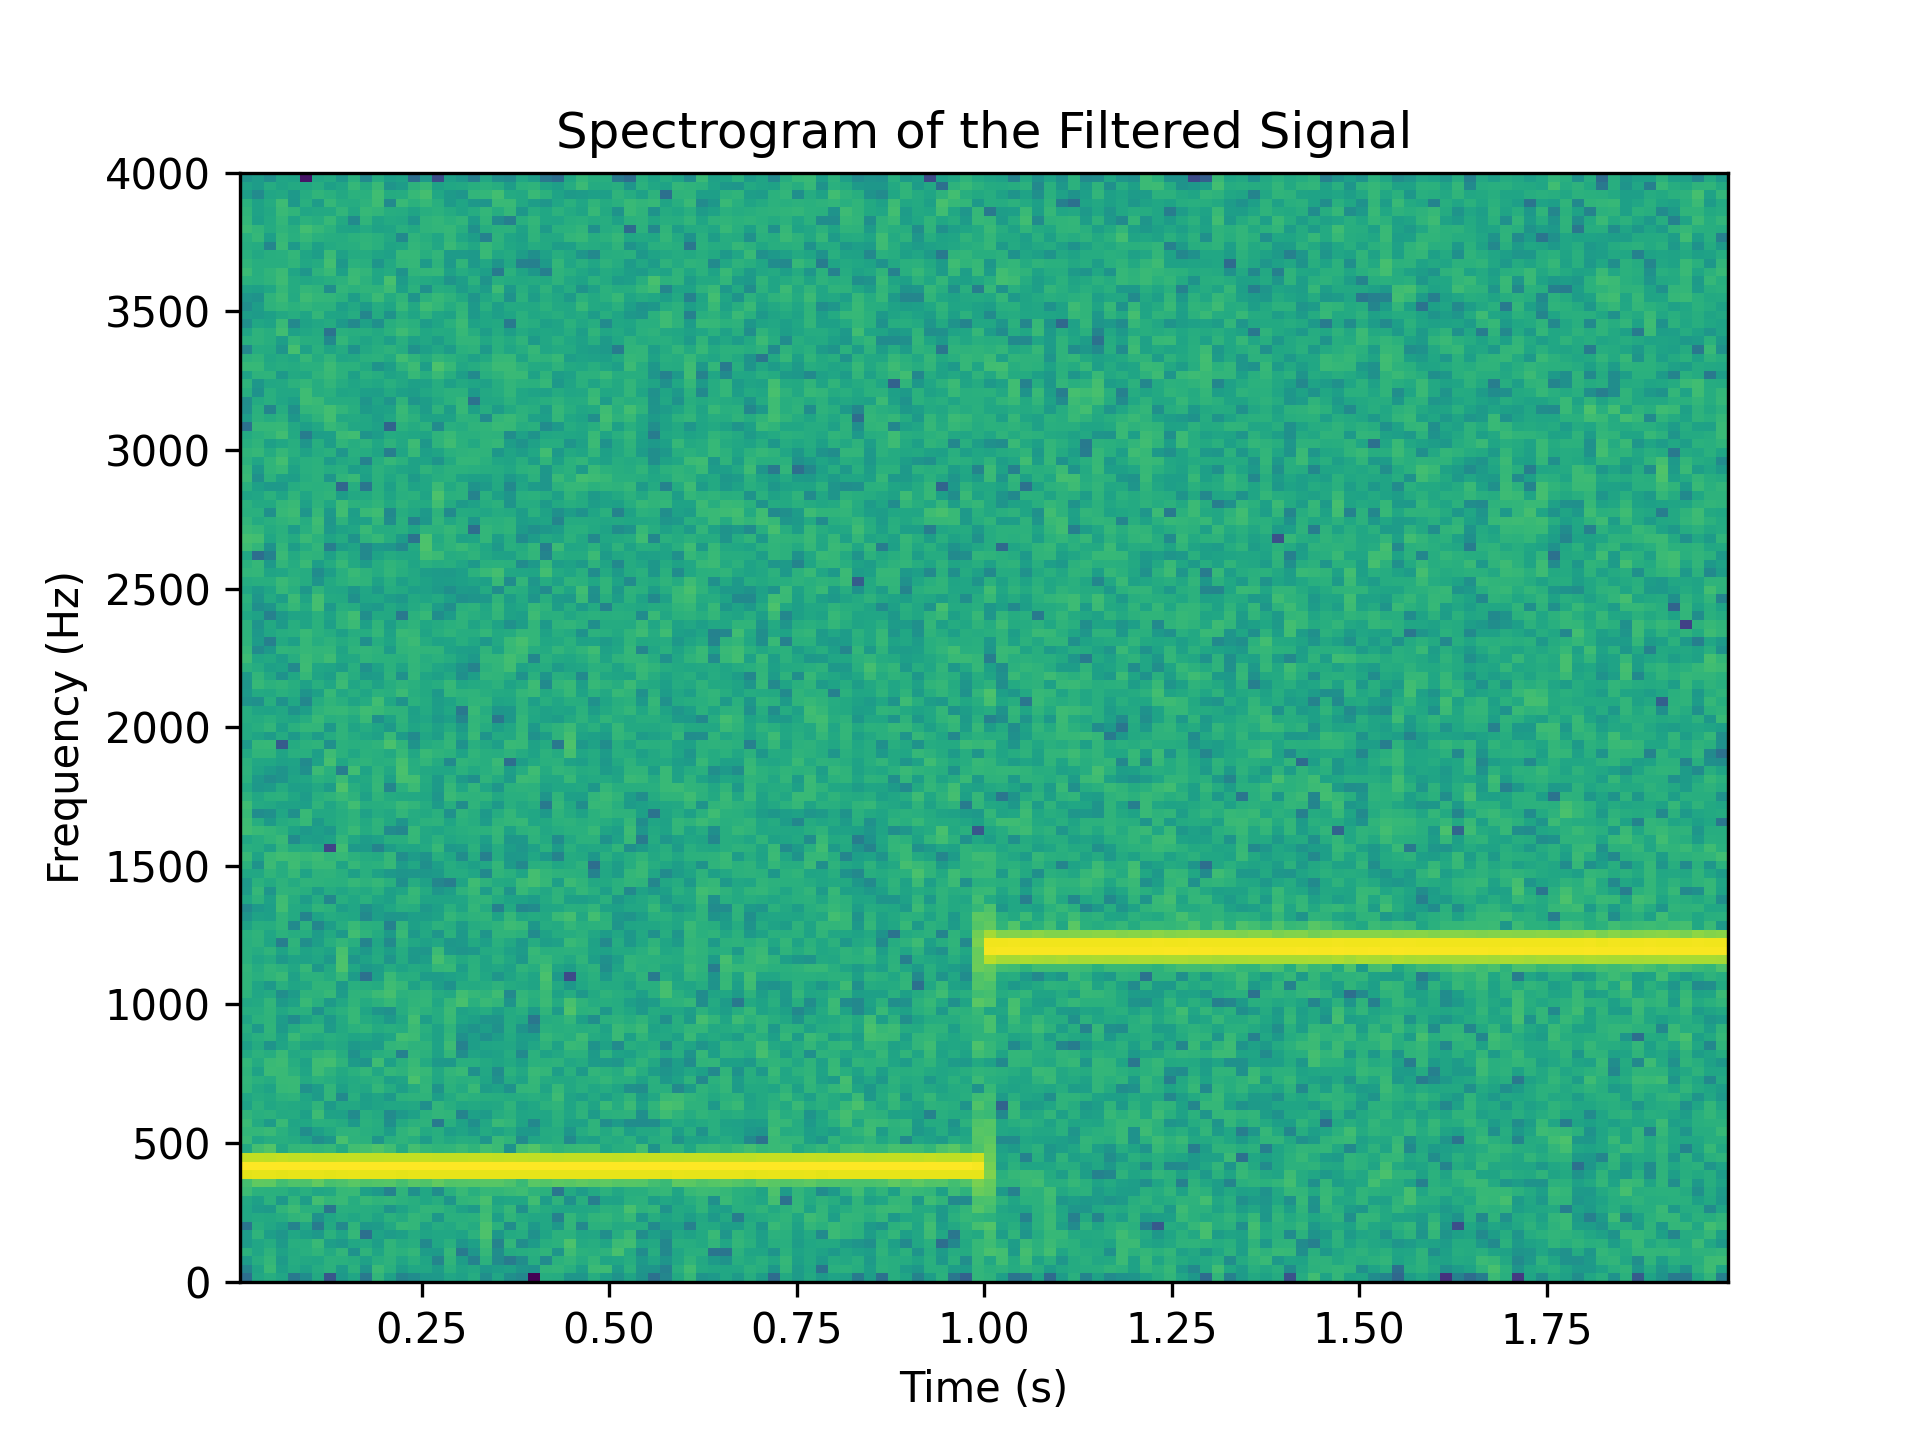
\includegraphics[width=0.5\columnwidth]{images/spectrogram_input.png}
    \caption{Spectrogram of input signal}
    \label{fig:input_spectrogram}
\end{figure}

\begin{figure}[ht]
    \centering
    % First figure
    \begin{minipage}{0.475\columnwidth}
        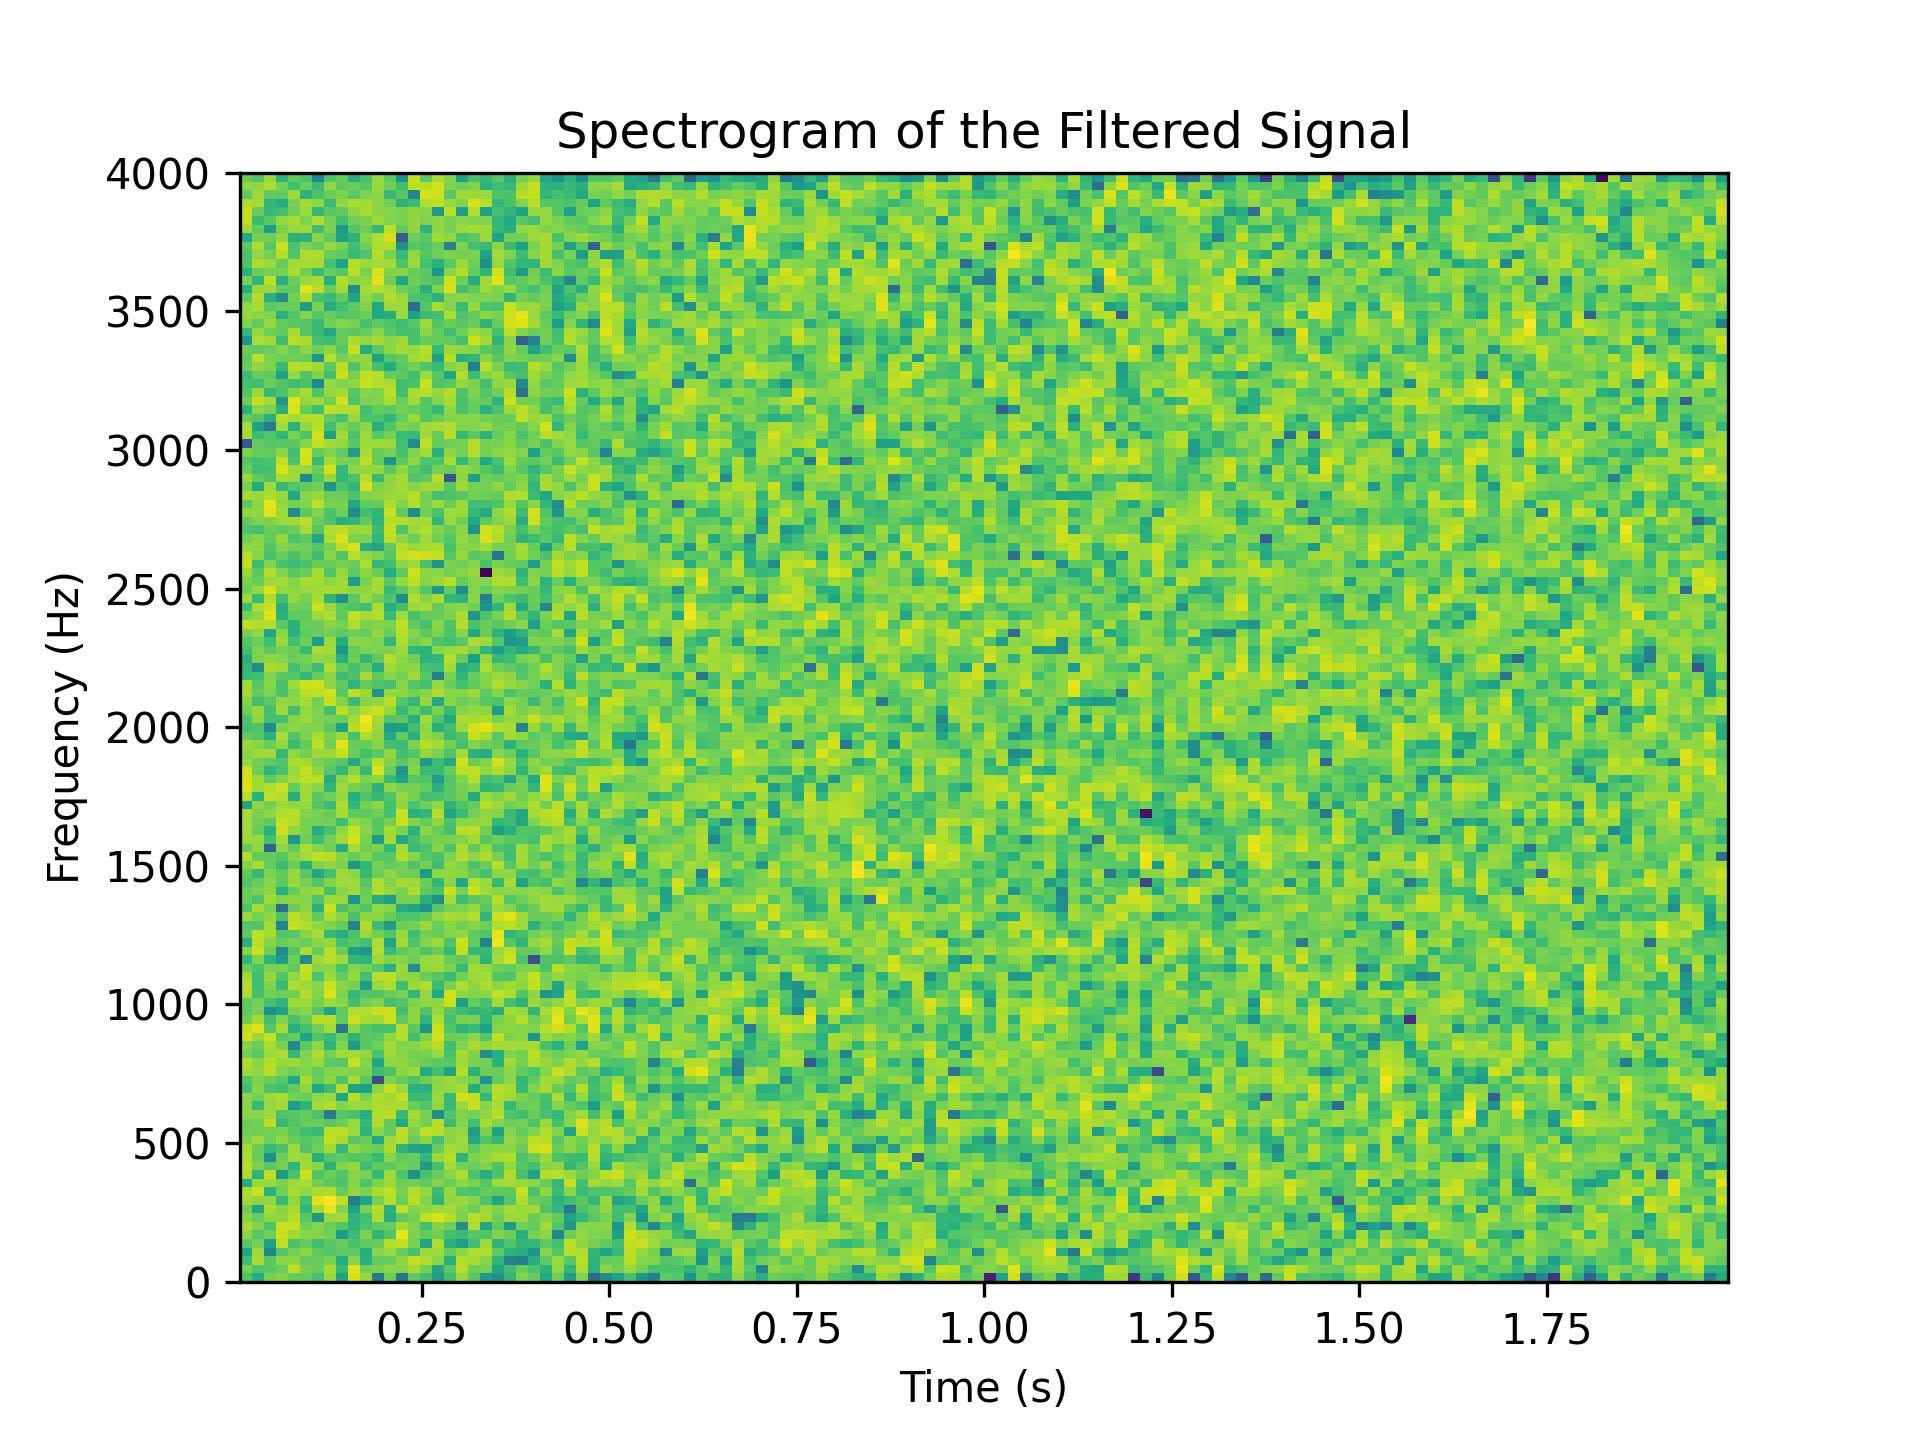
\includegraphics[width=\linewidth]{images/spectrogram_output_a_9.png}
        \label{fig:adaptive_assy_spectrogram_l9}
    \end{minipage}\hfill
    % Second figure
    \begin{minipage}{0.475\columnwidth}
        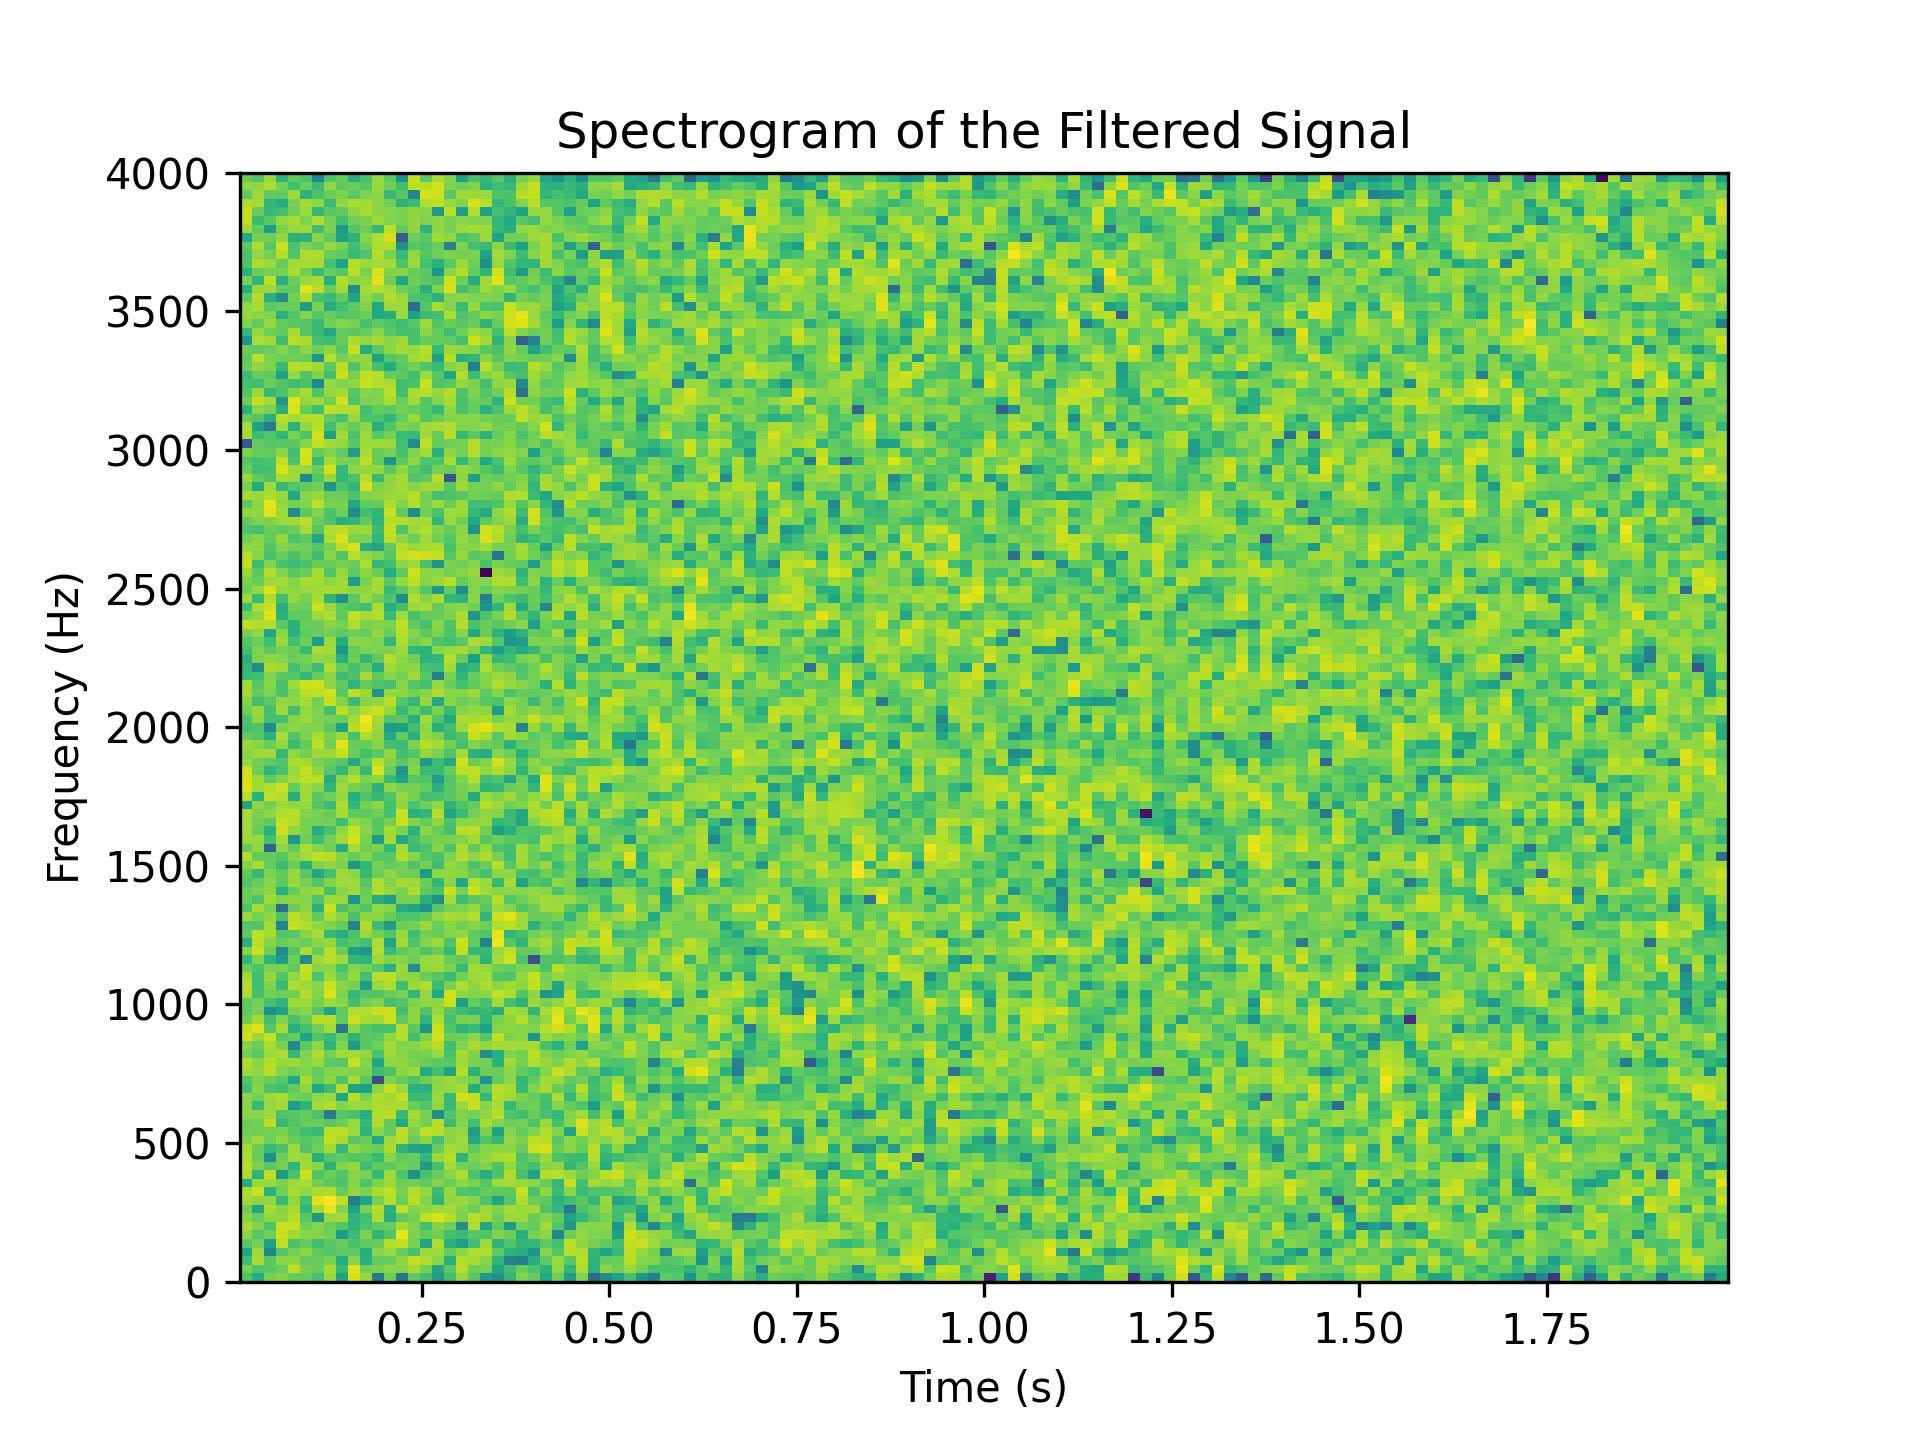
\includegraphics[width=\linewidth]{images/spectrogram_output_c_9.png}
    \end{minipage}\hfill
    \caption{Spectrogram of $2^{nd}$ order ANF with $\lambda = 0.9$ in C(left) and Assembler(right)}
    \label{fig:adaptive_c_spectrogram_l9}
\end{figure}



The setting of $\lambda = 0.9$  demonstrates significant noise reduction at 400 Hz and 1200 Hz. Comparable results from a C implementation (\autoref{fig:adaptive_c_spectrogram_l9}) were also presented .


For intuitive comparison, we plot the frequency responses of the input and the output signals from the ANF in both assembly and C (\autoref{fig:input_frequency_response}, \autoref{fig:adaptive_frequency_response}). These plots underscore the Adaptive $\rho$ mechanism, enhancing the convergence speed and tracking ability of the filter.

\begin{figure}[ht]
\centering
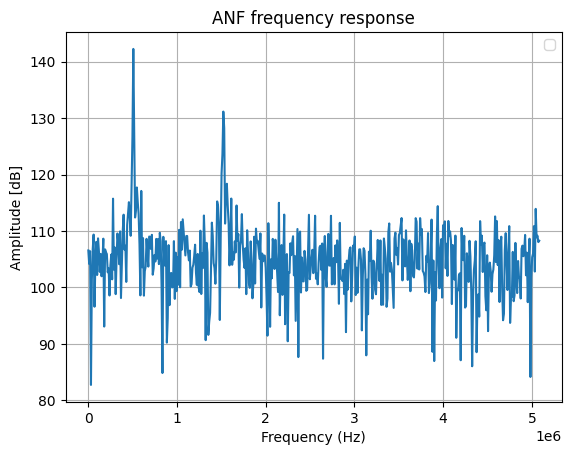
\includegraphics[width=0.5\columnwidth]{images/input_frequency_response.png}
\caption{Input frequency response}
\label{fig:input_frequency_response}
\end{figure}

Comparatively, the frequency responses after filtering (\autoref{fig:adaptive_frequency_response}) show the effective removal of the narrow band and high intensity frequency components at 400Hz and 1200Hz.

\begin{figure}[ht]
    \centering
    % First figure
    \begin{minipage}{0.475\columnwidth}
        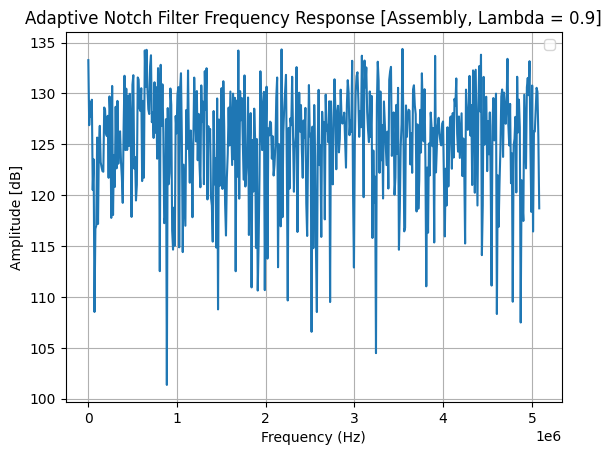
\includegraphics[width=\linewidth]{images/Adaptive_Notch_Filter_Assy_Frequency_Response_L9.png}
    \end{minipage}\hfill
    % Second figure
    \begin{minipage}{0.475\columnwidth}
        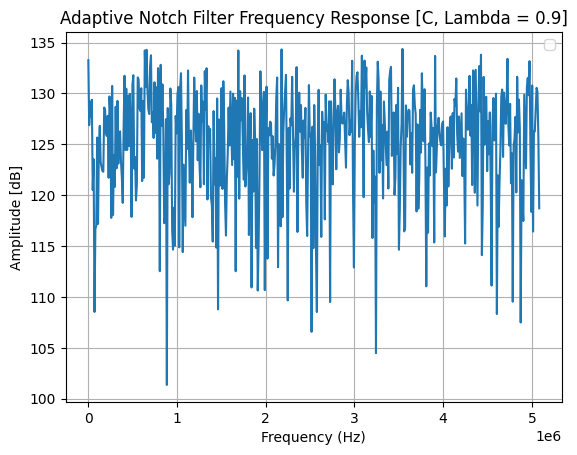
\includegraphics[width=\linewidth]{images/Adaptive_Notch_Filter_C_Frequency_Response.png}
    \end{minipage}\hfill
    \caption{Frequency Response of ANF with adaptive $\rho$ and $\lambda = 0.9$ in C(left) and Assembler(right)}
    \label{fig:adaptive_frequency_response}
\end{figure}


\subsection{Computational cost analysis}
The computational efficiency of our ANF implementations was quantified in terms of clock cycles, a direct measure of processing time. The results, as detailed in Table \ref{tab:comp_cost}, indicate that both the C and Assembler implementations have similar computational demands. This similarity suggests that our optimization strategies were effective across both programming languages, maintaining a balance between performance and computational resource utilization. 

However, it is noteworthy that even minor differences in clock cycles can have significant implications in resource-constrained environments. Therefore, future work will focus on further optimizing the computational efficiency of our ANF, particularly for deployment in embedded systems or platforms with stringent resource limitations.


\begin{table}[ht]
\centering
\begin{tabular}{l|l}
\hline
Implementation                     & Clock cycle \\ \hline
ANF with $\lambda = 0.9$ in C         & 16,733,840  \\
ANF with $\lambda = 0.9$ in Assembler & 16,733,632  \\
ANF with $\lambda = 0.9$ in C         & 16,733,519  \\
ANF with $\lambda = 0.9$ in Assembler & 16,733,377 \\ \hline
\end{tabular}
\caption{Computational cost (clock cycles) of all different implementation}
\label{tab:comp_cost}
\end{table}

